\section{Method}\label{sec:method}

This section explains the methods of sentiment analysis we designed in this project. Figure \ref{fig:method-steps} illustrates the method steps. First, \textit{preprocessing} is applied to the raw data files, which is described in Section \ref{sec:method:preprocessing}. Second, \textit{word-vector embeddings} are produced (cf. Section \ref{sec:method:embeddings}). Third and finally, a \textit{classification} algorithm is trained to acquire prediction capabilities, as explained in Section \ref{sec:method:classification}.

\begin{figure} 	
	\centering 	
	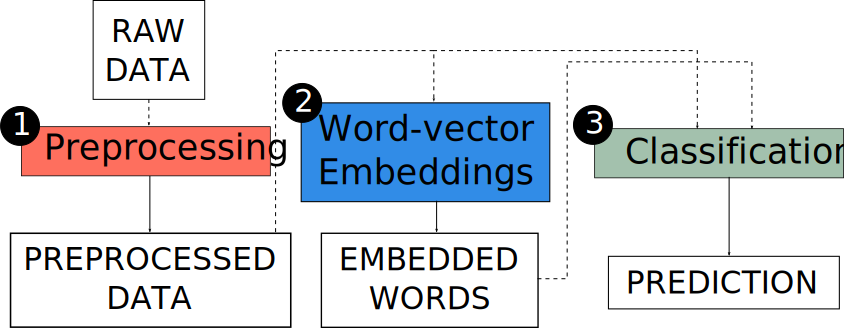
\includegraphics[width=\columnwidth]{graphics/method-steps.pdf} 	
	\caption{Illustration of method steps} 	
	\label{fig:method-steps} 
\end{figure}

\subsection{Preprocessing}\label{sec:method:preprocessing}
The given dataset presents a set of challenges which have to be addressed in order to extract meaningful data. First, the constraint of 140 characters gives rise to a plethora of abbreviations and acronyms. Second, orthography is not observed. We evaluated several methods to address at least some of these issues (as did Bao et al. \cite{bao2014role}).

All these methods aim to reduce the size of our dictionary. They either remove what we considered sentiment-neutral words, or they map differently spelled words onto one. Additionally, inspired by the papers \cite{hemalatha2012preprocessing} and \cite{bao2014role} we implemented the methods \textit{Same-Letter Sequence Removal} and \textit{Negation Connection}.

\subsubsection{Negation Replacement (N)}\label{sec:method:negation-replacement}

Negation replacement substitutes common negated terms with their opposite expressions.

\subsubsection{Word Cancellation (S)}\label{sec:method:word-cancellation}

Word Cancellation removes frequent words that we assumed to be sentiment-free. Examples include: '\textit{i}', '\textit{you}', '\textit{am}'. For the complete list, please contact the authors.

\subsubsection{Tag Removal (R)}\label{sec:method:tag-removal}

Tag removal eliminates the tags \textit{\textless user\textgreater} and \textit{\textless url\textgreater} from every tweet.

\subsubsection{Negation Connection (C) and Negation Disconnection (D)}\label{sec:method:negation-connection}
Negation connection implies that '\textit{n't}' becomes '\textit{nt}', whereas negation disconnection transforms '\textit{n't}' into ' \textit{not}'.

\subsubsection{Short Word Removal (3)}\label{sec:method:short-word-removal}

Short Word Removal removes a word if it consists of two characters or less.

\subsubsection{Same-Letter Sequence Removal (M)}\label{sec:method:same-letter-removal}

If the word contains a letter more than twice in a row, that sequence is shortened down to two characters. For instance, occurrences like '\textit{loool}' are shortened to '\textit{lool}'.

\subsubsection{Word Type Filtering (W)}\label{sec:method:word-type-filtering}

This method categorises every word and then keeps or discards it based on its type. Words were kept if they belonged to one of the types noun, verb, adverb, and adjective.

\subsection{Word embeddings}\label{sec:method:embeddings}

On the basis of preprocessed files, \textit{word-vector embeddings} are produced. Such embedding methods map each word in the vocabulary to a vector in a multi-dimensional space. Semantic relations between words should then be captured by geometric relations between the corresponding vectors, e.g., distance.

In this project, we used and evaluated two well-known embedding methods: \textit{GloVe} \cite{pennington2014glove} and \textit{word2vec} \cite{mikolov2013word2vec}. Coarsely put, both methods work by adapting vectors iteratively such that the dot product of two word vectors is proportional to the probability that the two respective words occur in the same context.

\subsection{Classification}\label{sec:method:classification}

Since a simple and effective approach to learn distributed representations of words was proposed \cite{mikolov2013word2vec}, neural networks advance sentiment analysis substantially.
	
The first such network models, among which are Recursive Neural Network (\cite{socher2011parsing, dong2014adaptive, qian2015learning}), Recursive Neural Tensor Networks (\cite{socher2013reasoning}), and Recurrent Neural Networks (\cite{mikolov2010recurrent}), performed sentiment analysis by utilizing syntax structures of sentences. However, such methods may suffer from syntax parsing errors. In addition, Recurrent Neural Networks (RNN) do not allow information to persist in the long-term. A common solution to this problem was given by LSTM (Long Short-Term Memory) networks, which contain special gates that control the information flow \cite{hochreiter1997long}. 
	
Since LSTM networks are capable of learning long-term dependencies, they are well-suited for natural language modeling. Furthermore, they are less prone to encounter gradient vanishing problems than RNN models. More formally, each cell in LSTM can be computed as follows:

\begin{align}
	X & =\begin{bmatrix}
	h_{t-1} \\
	x_{t} \\
	\end{bmatrix}\\	
	f_{t} & = \sigma(W_{f} \cdot X + b_{f} )  \\
	i_{t} & = \sigma(W_{i} \cdot X + b_{i} )  \\
	o_{t} & = \sigma(W_{o} \cdot X + b_{o} )  \\
	c_{t} & = f_{t} \odot c_{t-1} + i_{t} \odot \mathit{tanh}(W_{c}  \odot X + b_{c})\\
	h_{t} & = o_{t} \odot tanh(c_{t}),
\end{align}		
where $W_{f} , W_{i} , W_{o}, W_{c} \in {\rm I\!R}^{d\times(n + d)}$ are the weighted matrices and $ b_{f},  b_{i}, b_{o}, b_{c} \in {\rm I\!R}^{d}$ are biases to be learned during training, parameterizing the transformations of the input, forget and output gates, respectively. $\sigma$ is the sigmoid function and $\odot$ stands for element-wise multiplication. $ x_{t} \in {\rm I\!R}^{n}$ includes the inputs of LSTM cell unit, representing the word embedding vectors $w_{t}$ (cf. Figure \ref{fig:attention-mechanism}). The vector of hidden layer $t$ is $h_{t} \in {\rm I\!R}^{d}$, where $d$ is the number of hidden units in a cell. Then different approaches can be applied to obtain a vector representation of a sentence. The last hidden vector $h_{N}$ can be considered as the feature representation and also the average of the hidden vectors.

A fully connected hidden layer calculates the transformation $\delta(W_{s} ∗ h_{N} + b_{s})$, where $W_{s} \in {\rm I\!R}^{K,d}$ is the weight matrix, $b_{s} \in {\rm I\!R}^{K}$ the bias, and $\delta$ an  activation function such as the rectified linear unit or $\mathit{tanh}$. The output vector of this layer corresponds to logits that are normalized through a softmax function. Finally, the output returns the probabilities for each class, $y\in \{-1, 1\} $ and $K=2$.
	
A potential issue with this setup is that a neural network needs to be able to compress all the necessary information of a sentence into a fixed-length vector that is fed to the fully connected layer. Inspired by Bahdanau et al. \cite{AttentionBahdanau}, regarding machine translation, we propose to implement an attention mechanism that does not attempt to summarize a whole text into a single vector. Instead, it encodes the input sentence into a sequence of vectors and chooses a subset of these vectors adaptively. Each time that model generates a prediction, it searches for a set of positions in the sentence where the most relevant information is concentrated. Hence, the vector representation is based on the concatenation of the last hidden unit and the context vector computed as weighted sum of all the hidden units. Let $H \in {\rm I\!R}^{d\times N}$ be a matrix consisting of hidden vectors $[h_1, ... , h_N]$ that the LSTM produced, where $z$ is the size of hidden layers for the attention mechanism and $N$ is the length of the given sentence.	
\begin{align}
	M &= \mathit{tanh}(W_h \cdot H)\\
	\alpha &= \mathit{softmax}(w^{T} \cdot M)\\
	r &= H \cdot \alpha^T\\ h^* &= \mathit{tanh}(W_p \cdot  r + W_x \cdot h_N)\\
	y &= \mathit{softmax}(W_s \cdot  h^* + b_s),
\end{align}	
where $W_h \in {\rm I\!R}^{z\times d}, W_p \in {\rm I\!R}^{d\times d},  W_x \in {\rm I\!R}^{d\times d}, w \in {\rm I\!R}^{z}$ are the new matrices of parameters estimated by minimizing the cross-entropy error between $y$ and $\hat{y}$ for all sentences.
	
Luong et al. \cite{luong2015effective} proposed an interesting modification method by categorizing various attention-based models into two broad categories, global and local. The global attention described above computes the scores or alignment ($\alpha$) by taking into account all the hidden states from a sentence. On the other hand, the local attention offers a mechanism that focus on a smaller subsets of words. Compared to the suggested implementation stated in the original paper, we adapted the formulas to perform text classification tasks. In other words, the algorithm selects a window where the alignments decay exponentially around the center. More formally, our model predicts the midpoint of defined interval as follows:  
\begin{align}
	p_t &= N \cdot \mathit{sigmoid}(\upsilon_c \mathit{tanh}(W_c \cdot h_N))\\
	\alpha &= \mathit{softmax}(w^{T} \cdot M) \cdot \exp\bigg(-\frac{(s - p_t)^2}{2\sigma^2}\bigg).
\end{align}
		
$W_c,$  $\upsilon_c$ are the model parameters which will be learned to predict positions. $N$ is the source sentence length. As a result of sigmoid, $p_t \in [0, N]$. To favor alignment points near $p_t$, we place a Gaussian distribution centered around $p_t$. 

The network parameters are learned using Adam optimizer \cite{kingma2014adam}. We set the hyper-parameters to $\eta = 0.001$(learning rate), $\beta_1$ = 0.9, $\beta_2=0.999$ and we linearly decreased $\eta$ whenever the loss function did not improve in the previous 10'000 iterations with a batch size of 64. In Section \ref{sec:results}, we will assess the accuracy of each of those different architectures.

\begin{figure} 	
	\centering 	
	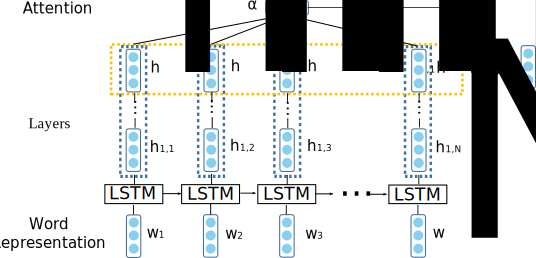
\includegraphics[width=\columnwidth]{graphics/attention-mechanism.pdf} 	
	\caption{Illustration of global attention mechanism} 	
	\label{fig:attention-mechanism} 
\end{figure}
